% Εισαγωγή

\addcontentsline{toc}{chapter}{Εισαγωγή}
\chapter*{Εισαγωγή}

Η υπολογιστική γεωμετρία είναι ο τομέας της επιστήμης της Πληροφορικής που αφορά τη μελέτη αλγορίθμων σχετικά με γεωμετρικά προβλήματα. Ο κυρίαρχος στόχος είναι η ανάπτυξη αποδοτικών αλγορίθμων και δομών δεδομένων για την επίλυση προβλημάτων σε γεωμετρικά αντικείμενα όπως τα διδιάστατα αρχέγονα, τα οποία δύναται να περιλαμβάνουν σημεία, γραμμές και ευθύγραμμα τμήματα, καθώς και πολύγωνα. Οι εφαρμογές της συνδυαστικής υπολογιστικής γεωμετρίας επεκτείνονται επίσης στη γραφική υπολογιστών, όπου βρίσκουν εφαρμογή στη σχεδίαση σχημάτων σε δύο διαστάσεις. \par

\vspace{0.5em}

\begin{figure}[h]
\centering
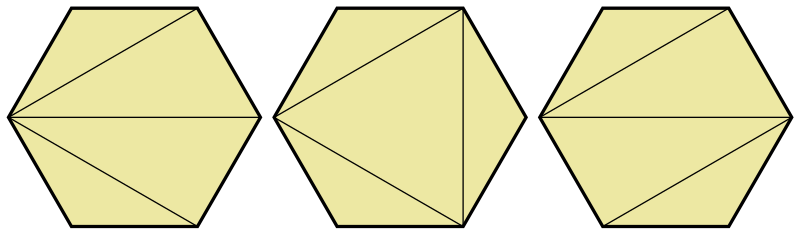
\includegraphics[width=0.5\textwidth]{images/polygons}
\caption{Πολύγωνα κατασκευασμένα από αρχέγονα}
\end{figure}

Η παρούσα εργασία αποτελεί προσπάθεια γενίκευσης και υλοποίησης της δοθείσας διαδικασίας \textlatin{triangle1} στην \textlatin{convex1}, η οποία χαράσσει αυθαίρετα κυρτά πολύγωνα, υπολογίζοντας αυξητικώς τις γραμμικές συναρτήσεις των ακμών τους για όλα τα εικονοστοιχεία του περιβάλλοντος κυτίου τους. Γενικώς τα τρίγωνα θεωρούνται αρχέγονα, διότι κάθε πολύγωνο δύναται να κατασκευαστεί από αυτά (Δρακόπουλος, 2021). Από πλευράς γεωμετρίας, ένα πολύγωνο (\textlatin{polygon}) είναι ένα επίπεδο σχήμα που ορίζεται από ένα σύνολο τριών ή περισσότερων θέσεων συντεταγμένων που ονομάζονται κορυφές (\textlatin{vertices}), και συνδέονται στη σειρά από ευθύγραμμα τμήματα που ονομάζονται ακμές (\textlatin{edges}) ή πλευρές (\textlatin{sides}) του πολυγώνου, οι οποίες δεν πρέπει να έχουν άλλα κοινά σημεία εκτός από τις κορυφές τους. Στην προκειμένη εργασία θα εξετάσουμε τα κυρτά πολύγωνα, τα οποία ορίζονται ως τα πολύγωνα των οποίων όλες οι εσωτερικές γωνίες είναι μικρότερες από ή ίσες με $180\degree$ (\textlatin{Hearn \& Baker, 2010}, σ. 117). \par

Η απεικόνιση των αρχεγόνων και κατ’ επέκταση των πολυγώνων γίνεται σε 2Δ συσκευές οθονών. Αυτές είναι διδιάστατες επιφάνειες πάνω στις οποίες προβάλλεται η οπτική πληροφορία ως ένα διακριτό πλέγμα εικονοστοιχείων. Η διαδικασία μετατροπής ενός 2Δ αρχεγόνου σε διακριτή αναπαράσταση εικονοστοιχείων, δηλαδή η εύρεση των εικονοστοιχείων  που απαρτίζουν ένα στοιχειώδες σχήμα, ονομάζεται ψηφιδόξυση ή χάραξη (\textlatin{rasterization}) (Δρακόπουλος, 2021?  Μουστάκας κ.ά., 2015? Σπύρου, 2019). \par
